% SOURCE: ../../edit-harness/results/merging/RG_gain_law_20260715.json
% !TEX encoding = UTF-8 Unicode
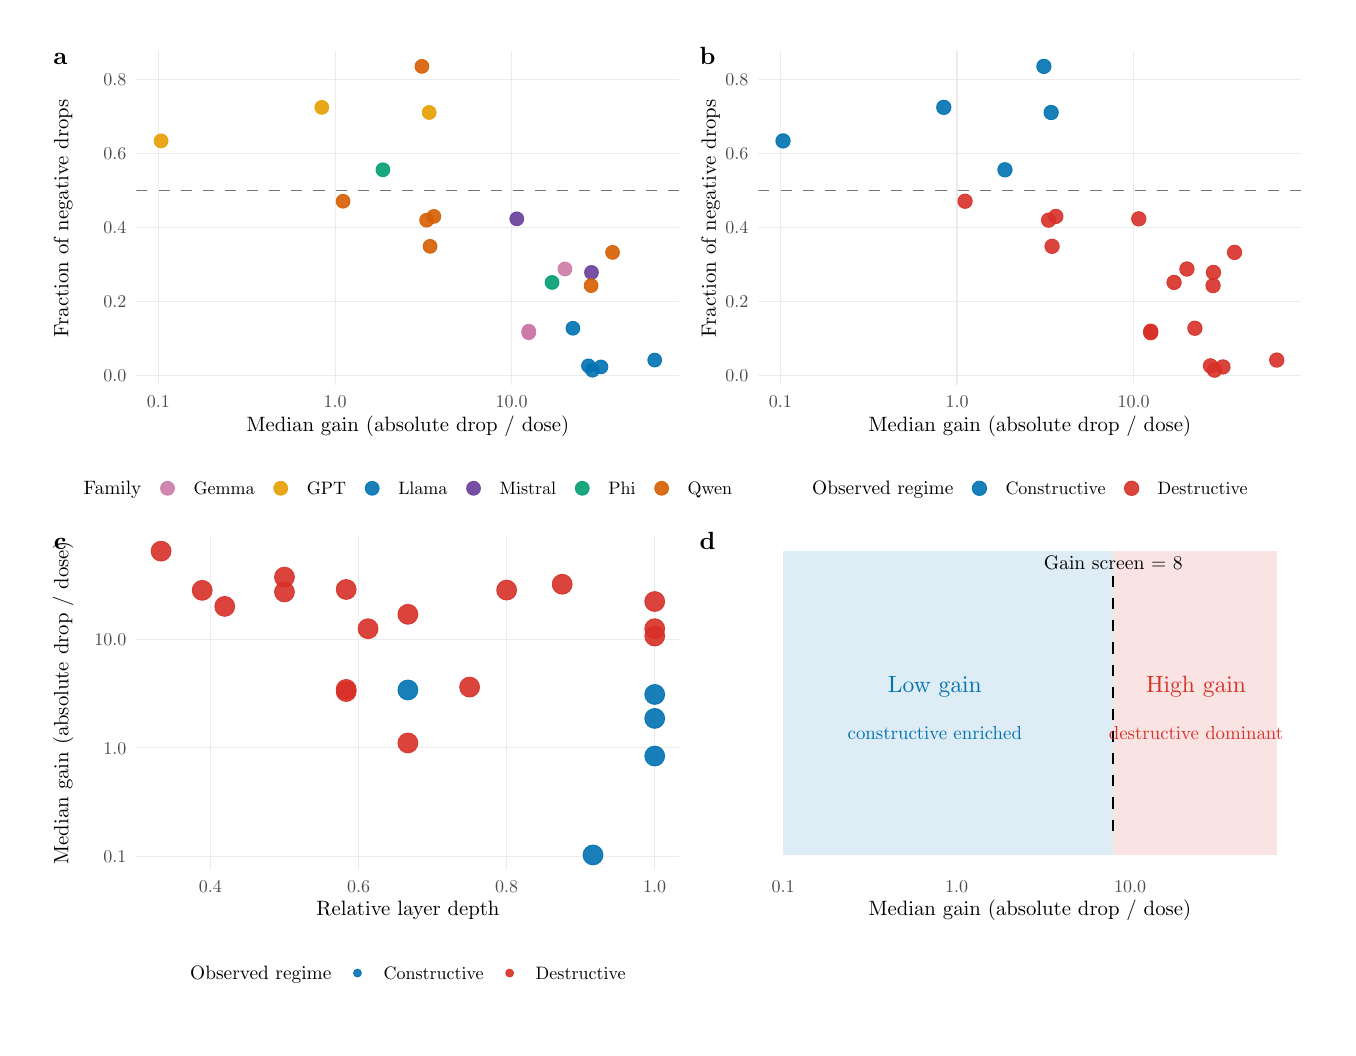
\begin{tikzpicture}[x=1pt,y=1pt]
\definecolor{fillColor}{RGB}{255,255,255}
\path[use as bounding box,fill=fillColor,fill opacity=0.00] (0,0) rectangle (469.75,361.35);
\begin{scope}
\path[clip] (  0.00,  0.00) rectangle (469.75,361.35);
\definecolor{drawColor}{RGB}{255,255,255}
\definecolor{fillColor}{RGB}{255,255,255}

\path[draw=drawColor,line width= 0.6pt,line join=round,line cap=round,fill=fillColor] (  0.00,  0.00) rectangle (469.75,361.35);
\end{scope}
\begin{scope}
\path[clip] (  5.50,180.68) rectangle (239.50,355.85);
\definecolor{fillColor}{RGB}{255,255,255}

\path[fill=fillColor] (  5.50,180.68) rectangle (239.50,355.85);
\end{scope}
\begin{scope}
\path[clip] (239.50,180.68) rectangle (464.25,355.85);
\definecolor{fillColor}{RGB}{255,255,255}

\path[fill=fillColor] (239.50,180.68) rectangle (464.25,355.85);
\end{scope}
\begin{scope}
\path[clip] (  5.50,  5.50) rectangle (239.50,180.68);
\definecolor{fillColor}{RGB}{255,255,255}

\path[fill=fillColor] (  5.50,  5.50) rectangle (239.50,180.68);
\end{scope}
\begin{scope}
\path[clip] (239.50,  5.50) rectangle (464.25,180.68);
\definecolor{fillColor}{RGB}{255,255,255}

\path[fill=fillColor] (239.50,  5.50) rectangle (464.25,180.68);
\end{scope}
\begin{scope}
\path[clip] ( 39.28,232.09) rectangle (235.50,352.85);
\definecolor{drawColor}{gray}{0.92}

\path[draw=drawColor,line width= 0.4pt,line join=round] ( 39.28,235.81) --
	(235.50,235.81);

\path[draw=drawColor,line width= 0.4pt,line join=round] ( 39.28,262.49) --
	(235.50,262.49);

\path[draw=drawColor,line width= 0.4pt,line join=round] ( 39.28,289.16) --
	(235.50,289.16);

\path[draw=drawColor,line width= 0.4pt,line join=round] ( 39.28,315.84) --
	(235.50,315.84);

\path[draw=drawColor,line width= 0.4pt,line join=round] ( 39.28,342.52) --
	(235.50,342.52);

\path[draw=drawColor,line width= 0.4pt,line join=round] ( 47.24,232.09) --
	( 47.24,352.85);

\path[draw=drawColor,line width= 0.4pt,line join=round] (111.07,232.09) --
	(111.07,352.85);

\path[draw=drawColor,line width= 0.4pt,line join=round] (174.90,232.09) --
	(174.90,352.85);
\definecolor{drawColor}{gray}{0.45}

\path[draw=drawColor,line width= 0.3pt,dash pattern=on 4pt off 4pt ,line join=round] ( 39.28,302.50) -- (235.50,302.50);
\definecolor{drawColor}{RGB}{0,114,178}
\definecolor{fillColor}{RGB}{0,114,178}

\path[draw=drawColor,draw opacity=0.90,line width= 0.3pt,line join=round,line cap=round,fill=fillColor,fill opacity=0.90] (197.02,252.73) circle (  2.51);

\path[draw=drawColor,draw opacity=0.90,line width= 0.3pt,line join=round,line cap=round,fill=fillColor,fill opacity=0.90] (202.64,239.14) circle (  2.51);

\path[draw=drawColor,draw opacity=0.90,line width= 0.3pt,line join=round,line cap=round,fill=fillColor,fill opacity=0.90] (204.09,237.58) circle (  2.51);

\path[draw=drawColor,draw opacity=0.90,line width= 0.3pt,line join=round,line cap=round,fill=fillColor,fill opacity=0.90] (226.58,241.24) circle (  2.51);

\path[draw=drawColor,draw opacity=0.90,line width= 0.3pt,line join=round,line cap=round,fill=fillColor,fill opacity=0.90] (207.15,238.76) circle (  2.51);
\definecolor{drawColor}{RGB}{106,61,154}
\definecolor{fillColor}{RGB}{106,61,154}

\path[draw=drawColor,draw opacity=0.90,line width= 0.3pt,line join=round,line cap=round,fill=fillColor,fill opacity=0.90] (203.73,272.90) circle (  2.51);

\path[draw=drawColor,draw opacity=0.90,line width= 0.3pt,line join=round,line cap=round,fill=fillColor,fill opacity=0.90] (176.74,292.27) circle (  2.51);
\definecolor{drawColor}{RGB}{0,158,115}
\definecolor{fillColor}{RGB}{0,158,115}

\path[draw=drawColor,draw opacity=0.90,line width= 0.3pt,line join=round,line cap=round,fill=fillColor,fill opacity=0.90] (189.49,269.29) circle (  2.51);

\path[draw=drawColor,draw opacity=0.90,line width= 0.3pt,line join=round,line cap=round,fill=fillColor,fill opacity=0.90] (128.37,309.99) circle (  2.51);
\definecolor{drawColor}{RGB}{213,94,0}
\definecolor{fillColor}{RGB}{213,94,0}

\path[draw=drawColor,draw opacity=0.90,line width= 0.3pt,line join=round,line cap=round,fill=fillColor,fill opacity=0.90] (203.59,268.14) circle (  2.51);

\path[draw=drawColor,draw opacity=0.90,line width= 0.3pt,line join=round,line cap=round,fill=fillColor,fill opacity=0.90] (144.16,291.79) circle (  2.51);

\path[draw=drawColor,draw opacity=0.90,line width= 0.3pt,line join=round,line cap=round,fill=fillColor,fill opacity=0.90] (113.97,298.63) circle (  2.51);

\path[draw=drawColor,draw opacity=0.90,line width= 0.3pt,line join=round,line cap=round,fill=fillColor,fill opacity=0.90] (142.45,347.36) circle (  2.51);

\path[draw=drawColor,draw opacity=0.90,line width= 0.3pt,line join=round,line cap=round,fill=fillColor,fill opacity=0.90] (211.35,280.15) circle (  2.51);

\path[draw=drawColor,draw opacity=0.90,line width= 0.3pt,line join=round,line cap=round,fill=fillColor,fill opacity=0.90] (146.77,293.14) circle (  2.51);

\path[draw=drawColor,draw opacity=0.90,line width= 0.3pt,line join=round,line cap=round,fill=fillColor,fill opacity=0.90] (145.41,282.33) circle (  2.51);
\definecolor{drawColor}{RGB}{204,121,167}
\definecolor{fillColor}{RGB}{204,121,167}

\path[draw=drawColor,draw opacity=0.90,line width= 0.3pt,line join=round,line cap=round,fill=fillColor,fill opacity=0.90] (194.14,274.14) circle (  2.51);

\path[draw=drawColor,draw opacity=0.90,line width= 0.3pt,line join=round,line cap=round,fill=fillColor,fill opacity=0.90] (181.05,251.11) circle (  2.51);

\path[draw=drawColor,draw opacity=0.90,line width= 0.3pt,line join=round,line cap=round,fill=fillColor,fill opacity=0.90] (181.07,251.68) circle (  2.51);
\definecolor{drawColor}{RGB}{230,159,0}
\definecolor{fillColor}{RGB}{230,159,0}

\path[draw=drawColor,draw opacity=0.90,line width= 0.3pt,line join=round,line cap=round,fill=fillColor,fill opacity=0.90] ( 48.20,320.43) circle (  2.51);

\path[draw=drawColor,draw opacity=0.90,line width= 0.3pt,line join=round,line cap=round,fill=fillColor,fill opacity=0.90] (145.08,330.70) circle (  2.51);

\path[draw=drawColor,draw opacity=0.90,line width= 0.3pt,line join=round,line cap=round,fill=fillColor,fill opacity=0.90] (106.28,332.55) circle (  2.51);
\end{scope}
\begin{scope}
\path[clip] (  0.00,  0.00) rectangle (469.75,361.35);
\definecolor{drawColor}{gray}{0.30}

\node[text=drawColor,anchor=base east,inner sep=0pt, outer sep=0pt, scale=  0.65] at ( 35.68,233.57) {0.0};

\node[text=drawColor,anchor=base east,inner sep=0pt, outer sep=0pt, scale=  0.65] at ( 35.68,260.25) {0.2};

\node[text=drawColor,anchor=base east,inner sep=0pt, outer sep=0pt, scale=  0.65] at ( 35.68,286.92) {0.4};

\node[text=drawColor,anchor=base east,inner sep=0pt, outer sep=0pt, scale=  0.65] at ( 35.68,313.60) {0.6};

\node[text=drawColor,anchor=base east,inner sep=0pt, outer sep=0pt, scale=  0.65] at ( 35.68,340.28) {0.8};
\end{scope}
\begin{scope}
\path[clip] (  0.00,  0.00) rectangle (469.75,361.35);
\definecolor{drawColor}{gray}{0.30}

\node[text=drawColor,anchor=base,inner sep=0pt, outer sep=0pt, scale=  0.65] at ( 47.24,224.02) {0.1};

\node[text=drawColor,anchor=base,inner sep=0pt, outer sep=0pt, scale=  0.65] at (111.07,224.02) {1.0};

\node[text=drawColor,anchor=base,inner sep=0pt, outer sep=0pt, scale=  0.65] at (174.90,224.02) {10.0};
\end{scope}
\begin{scope}
\path[clip] (  0.00,  0.00) rectangle (469.75,361.35);
\definecolor{drawColor}{RGB}{0,0,0}

\node[text=drawColor,anchor=base,inner sep=0pt, outer sep=0pt, scale=  0.75] at (137.39,215.59) {Median gain (absolute drop / dose)};
\end{scope}
\begin{scope}
\path[clip] (  0.00,  0.00) rectangle (469.75,361.35);
\definecolor{drawColor}{RGB}{0,0,0}

\node[text=drawColor,rotate= 90.00,anchor=base,inner sep=0pt, outer sep=0pt, scale=  0.75] at ( 14.67,292.47) {Fraction of negative drops};
\end{scope}
\begin{scope}
\path[clip] (  0.00,  0.00) rectangle (469.75,361.35);
\definecolor{drawColor}{RGB}{0,0,0}

\node[text=drawColor,anchor=base west,inner sep=0pt, outer sep=0pt, scale=  0.70] at ( 20.21,192.49) {Family};
\end{scope}
\begin{scope}
\path[clip] (  0.00,  0.00) rectangle (469.75,361.35);
\definecolor{drawColor}{RGB}{204,121,167}
\definecolor{fillColor}{RGB}{204,121,167}

\path[draw=drawColor,draw opacity=0.90,line width= 0.3pt,line join=round,line cap=round,fill=fillColor,fill opacity=0.90] ( 50.53,194.90) circle (  2.51);
\end{scope}
\begin{scope}
\path[clip] (  0.00,  0.00) rectangle (469.75,361.35);
\definecolor{drawColor}{RGB}{230,159,0}
\definecolor{fillColor}{RGB}{230,159,0}

\path[draw=drawColor,draw opacity=0.90,line width= 0.3pt,line join=round,line cap=round,fill=fillColor,fill opacity=0.90] ( 91.44,194.90) circle (  2.51);
\end{scope}
\begin{scope}
\path[clip] (  0.00,  0.00) rectangle (469.75,361.35);
\definecolor{drawColor}{RGB}{0,114,178}
\definecolor{fillColor}{RGB}{0,114,178}

\path[draw=drawColor,draw opacity=0.90,line width= 0.3pt,line join=round,line cap=round,fill=fillColor,fill opacity=0.90] (124.49,194.90) circle (  2.51);
\end{scope}
\begin{scope}
\path[clip] (  0.00,  0.00) rectangle (469.75,361.35);
\definecolor{drawColor}{RGB}{106,61,154}
\definecolor{fillColor}{RGB}{106,61,154}

\path[draw=drawColor,draw opacity=0.90,line width= 0.3pt,line join=round,line cap=round,fill=fillColor,fill opacity=0.90] (161.11,194.90) circle (  2.51);
\end{scope}
\begin{scope}
\path[clip] (  0.00,  0.00) rectangle (469.75,361.35);
\definecolor{drawColor}{RGB}{0,158,115}
\definecolor{fillColor}{RGB}{0,158,115}

\path[draw=drawColor,draw opacity=0.90,line width= 0.3pt,line join=round,line cap=round,fill=fillColor,fill opacity=0.90] (200.40,194.90) circle (  2.51);
\end{scope}
\begin{scope}
\path[clip] (  0.00,  0.00) rectangle (469.75,361.35);
\definecolor{drawColor}{RGB}{213,94,0}
\definecolor{fillColor}{RGB}{213,94,0}

\path[draw=drawColor,draw opacity=0.90,line width= 0.3pt,line join=round,line cap=round,fill=fillColor,fill opacity=0.90] (229.08,194.90) circle (  2.51);
\end{scope}
\begin{scope}
\path[clip] (  0.00,  0.00) rectangle (469.75,361.35);
\definecolor{drawColor}{RGB}{0,0,0}

\node[text=drawColor,anchor=base west,inner sep=0pt, outer sep=0pt, scale=  0.65] at ( 59.95,192.66) {Gemma};
\end{scope}
\begin{scope}
\path[clip] (  0.00,  0.00) rectangle (469.75,361.35);
\definecolor{drawColor}{RGB}{0,0,0}

\node[text=drawColor,anchor=base west,inner sep=0pt, outer sep=0pt, scale=  0.65] at (100.86,192.66) {GPT};
\end{scope}
\begin{scope}
\path[clip] (  0.00,  0.00) rectangle (469.75,361.35);
\definecolor{drawColor}{RGB}{0,0,0}

\node[text=drawColor,anchor=base west,inner sep=0pt, outer sep=0pt, scale=  0.65] at (133.91,192.66) {Llama};
\end{scope}
\begin{scope}
\path[clip] (  0.00,  0.00) rectangle (469.75,361.35);
\definecolor{drawColor}{RGB}{0,0,0}

\node[text=drawColor,anchor=base west,inner sep=0pt, outer sep=0pt, scale=  0.65] at (170.53,192.66) {Mistral};
\end{scope}
\begin{scope}
\path[clip] (  0.00,  0.00) rectangle (469.75,361.35);
\definecolor{drawColor}{RGB}{0,0,0}

\node[text=drawColor,anchor=base west,inner sep=0pt, outer sep=0pt, scale=  0.65] at (209.82,192.66) {Phi};
\end{scope}
\begin{scope}
\path[clip] (  0.00,  0.00) rectangle (469.75,361.35);
\definecolor{drawColor}{RGB}{0,0,0}

\node[text=drawColor,anchor=base west,inner sep=0pt, outer sep=0pt, scale=  0.65] at (238.50,192.66) {Qwen};
\end{scope}
\begin{scope}
\path[clip] (  0.00,  0.00) rectangle (469.75,361.35);
\definecolor{drawColor}{RGB}{0,0,0}

\node[text=drawColor,anchor=base,inner sep=0pt, outer sep=0pt, scale=  0.90] at ( 11.76,348.05) {\bfseries a};
\end{scope}
\begin{scope}
\path[clip] (264.03,232.09) rectangle (460.25,352.85);
\definecolor{drawColor}{gray}{0.92}

\path[draw=drawColor,line width= 0.4pt,line join=round] (264.03,235.81) --
	(460.25,235.81);

\path[draw=drawColor,line width= 0.4pt,line join=round] (264.03,262.49) --
	(460.25,262.49);

\path[draw=drawColor,line width= 0.4pt,line join=round] (264.03,289.16) --
	(460.25,289.16);

\path[draw=drawColor,line width= 0.4pt,line join=round] (264.03,315.84) --
	(460.25,315.84);

\path[draw=drawColor,line width= 0.4pt,line join=round] (264.03,342.52) --
	(460.25,342.52);

\path[draw=drawColor,line width= 0.4pt,line join=round] (271.99,232.09) --
	(271.99,352.85);

\path[draw=drawColor,line width= 0.4pt,line join=round] (335.82,232.09) --
	(335.82,352.85);

\path[draw=drawColor,line width= 0.4pt,line join=round] (399.65,232.09) --
	(399.65,352.85);
\definecolor{drawColor}{gray}{0.45}

\path[draw=drawColor,line width= 0.3pt,dash pattern=on 4pt off 4pt ,line join=round] (264.03,302.50) -- (460.25,302.50);
\definecolor{drawColor}{RGB}{215,48,39}
\definecolor{fillColor}{RGB}{215,48,39}

\path[draw=drawColor,draw opacity=0.90,line width= 0.3pt,line join=round,line cap=round,fill=fillColor,fill opacity=0.90] (421.77,252.73) circle (  2.61);

\path[draw=drawColor,draw opacity=0.90,line width= 0.3pt,line join=round,line cap=round,fill=fillColor,fill opacity=0.90] (427.40,239.14) circle (  2.61);

\path[draw=drawColor,draw opacity=0.90,line width= 0.3pt,line join=round,line cap=round,fill=fillColor,fill opacity=0.90] (428.84,237.58) circle (  2.61);

\path[draw=drawColor,draw opacity=0.90,line width= 0.3pt,line join=round,line cap=round,fill=fillColor,fill opacity=0.90] (451.34,241.24) circle (  2.61);

\path[draw=drawColor,draw opacity=0.90,line width= 0.3pt,line join=round,line cap=round,fill=fillColor,fill opacity=0.90] (431.90,238.76) circle (  2.61);

\path[draw=drawColor,draw opacity=0.90,line width= 0.3pt,line join=round,line cap=round,fill=fillColor,fill opacity=0.90] (428.48,272.90) circle (  2.61);

\path[draw=drawColor,draw opacity=0.90,line width= 0.3pt,line join=round,line cap=round,fill=fillColor,fill opacity=0.90] (401.49,292.27) circle (  2.61);

\path[draw=drawColor,draw opacity=0.90,line width= 0.3pt,line join=round,line cap=round,fill=fillColor,fill opacity=0.90] (414.24,269.29) circle (  2.61);
\definecolor{drawColor}{RGB}{0,114,178}
\definecolor{fillColor}{RGB}{0,114,178}

\path[draw=drawColor,draw opacity=0.90,line width= 0.3pt,line join=round,line cap=round,fill=fillColor,fill opacity=0.90] (353.13,309.99) circle (  2.61);
\definecolor{drawColor}{RGB}{215,48,39}
\definecolor{fillColor}{RGB}{215,48,39}

\path[draw=drawColor,draw opacity=0.90,line width= 0.3pt,line join=round,line cap=round,fill=fillColor,fill opacity=0.90] (428.34,268.14) circle (  2.61);

\path[draw=drawColor,draw opacity=0.90,line width= 0.3pt,line join=round,line cap=round,fill=fillColor,fill opacity=0.90] (368.91,291.79) circle (  2.61);

\path[draw=drawColor,draw opacity=0.90,line width= 0.3pt,line join=round,line cap=round,fill=fillColor,fill opacity=0.90] (338.72,298.63) circle (  2.61);
\definecolor{drawColor}{RGB}{0,114,178}
\definecolor{fillColor}{RGB}{0,114,178}

\path[draw=drawColor,draw opacity=0.90,line width= 0.3pt,line join=round,line cap=round,fill=fillColor,fill opacity=0.90] (367.20,347.36) circle (  2.61);
\definecolor{drawColor}{RGB}{215,48,39}
\definecolor{fillColor}{RGB}{215,48,39}

\path[draw=drawColor,draw opacity=0.90,line width= 0.3pt,line join=round,line cap=round,fill=fillColor,fill opacity=0.90] (436.10,280.15) circle (  2.61);

\path[draw=drawColor,draw opacity=0.90,line width= 0.3pt,line join=round,line cap=round,fill=fillColor,fill opacity=0.90] (371.52,293.14) circle (  2.61);

\path[draw=drawColor,draw opacity=0.90,line width= 0.3pt,line join=round,line cap=round,fill=fillColor,fill opacity=0.90] (370.16,282.33) circle (  2.61);

\path[draw=drawColor,draw opacity=0.90,line width= 0.3pt,line join=round,line cap=round,fill=fillColor,fill opacity=0.90] (418.89,274.14) circle (  2.61);

\path[draw=drawColor,draw opacity=0.90,line width= 0.3pt,line join=round,line cap=round,fill=fillColor,fill opacity=0.90] (405.80,251.11) circle (  2.61);

\path[draw=drawColor,draw opacity=0.90,line width= 0.3pt,line join=round,line cap=round,fill=fillColor,fill opacity=0.90] (405.82,251.68) circle (  2.61);
\definecolor{drawColor}{RGB}{0,114,178}
\definecolor{fillColor}{RGB}{0,114,178}

\path[draw=drawColor,draw opacity=0.90,line width= 0.3pt,line join=round,line cap=round,fill=fillColor,fill opacity=0.90] (272.95,320.43) circle (  2.61);

\path[draw=drawColor,draw opacity=0.90,line width= 0.3pt,line join=round,line cap=round,fill=fillColor,fill opacity=0.90] (369.83,330.70) circle (  2.61);

\path[draw=drawColor,draw opacity=0.90,line width= 0.3pt,line join=round,line cap=round,fill=fillColor,fill opacity=0.90] (331.03,332.55) circle (  2.61);
\end{scope}
\begin{scope}
\path[clip] (  0.00,  0.00) rectangle (469.75,361.35);
\definecolor{drawColor}{gray}{0.30}

\node[text=drawColor,anchor=base east,inner sep=0pt, outer sep=0pt, scale=  0.65] at (260.43,233.57) {0.0};

\node[text=drawColor,anchor=base east,inner sep=0pt, outer sep=0pt, scale=  0.65] at (260.43,260.25) {0.2};

\node[text=drawColor,anchor=base east,inner sep=0pt, outer sep=0pt, scale=  0.65] at (260.43,286.92) {0.4};

\node[text=drawColor,anchor=base east,inner sep=0pt, outer sep=0pt, scale=  0.65] at (260.43,313.60) {0.6};

\node[text=drawColor,anchor=base east,inner sep=0pt, outer sep=0pt, scale=  0.65] at (260.43,340.28) {0.8};
\end{scope}
\begin{scope}
\path[clip] (  0.00,  0.00) rectangle (469.75,361.35);
\definecolor{drawColor}{gray}{0.30}

\node[text=drawColor,anchor=base,inner sep=0pt, outer sep=0pt, scale=  0.65] at (271.99,224.02) {0.1};

\node[text=drawColor,anchor=base,inner sep=0pt, outer sep=0pt, scale=  0.65] at (335.82,224.02) {1.0};

\node[text=drawColor,anchor=base,inner sep=0pt, outer sep=0pt, scale=  0.65] at (399.65,224.02) {10.0};
\end{scope}
\begin{scope}
\path[clip] (  0.00,  0.00) rectangle (469.75,361.35);
\definecolor{drawColor}{RGB}{0,0,0}

\node[text=drawColor,anchor=base,inner sep=0pt, outer sep=0pt, scale=  0.75] at (362.14,215.59) {Median gain (absolute drop / dose)};
\end{scope}
\begin{scope}
\path[clip] (  0.00,  0.00) rectangle (469.75,361.35);
\definecolor{drawColor}{RGB}{0,0,0}

\node[text=drawColor,rotate= 90.00,anchor=base,inner sep=0pt, outer sep=0pt, scale=  0.75] at (248.67,292.47) {Fraction of negative drops};
\end{scope}
\begin{scope}
\path[clip] (  0.00,  0.00) rectangle (469.75,361.35);
\definecolor{drawColor}{RGB}{0,0,0}

\node[text=drawColor,anchor=base west,inner sep=0pt, outer sep=0pt, scale=  0.70] at (283.49,192.49) {Observed regime};
\end{scope}
\begin{scope}
\path[clip] (  0.00,  0.00) rectangle (469.75,361.35);
\definecolor{drawColor}{RGB}{0,114,178}
\definecolor{fillColor}{RGB}{0,114,178}

\path[draw=drawColor,draw opacity=0.90,line width= 0.3pt,line join=round,line cap=round,fill=fillColor,fill opacity=0.90] (343.92,194.90) circle (  2.61);
\end{scope}
\begin{scope}
\path[clip] (  0.00,  0.00) rectangle (469.75,361.35);
\definecolor{drawColor}{RGB}{215,48,39}
\definecolor{fillColor}{RGB}{215,48,39}

\path[draw=drawColor,draw opacity=0.90,line width= 0.3pt,line join=round,line cap=round,fill=fillColor,fill opacity=0.90] (398.92,194.90) circle (  2.61);
\end{scope}
\begin{scope}
\path[clip] (  0.00,  0.00) rectangle (469.75,361.35);
\definecolor{drawColor}{RGB}{0,0,0}

\node[text=drawColor,anchor=base west,inner sep=0pt, outer sep=0pt, scale=  0.65] at (353.34,192.66) {Constructive};
\end{scope}
\begin{scope}
\path[clip] (  0.00,  0.00) rectangle (469.75,361.35);
\definecolor{drawColor}{RGB}{0,0,0}

\node[text=drawColor,anchor=base west,inner sep=0pt, outer sep=0pt, scale=  0.65] at (408.34,192.66) {Destructive};
\end{scope}
\begin{scope}
\path[clip] (  0.00,  0.00) rectangle (469.75,361.35);
\definecolor{drawColor}{RGB}{0,0,0}

\node[text=drawColor,anchor=base,inner sep=0pt, outer sep=0pt, scale=  0.90] at (245.67,348.05) {\bfseries b};
\end{scope}
\begin{scope}
\path[clip] ( 39.28, 56.92) rectangle (235.50,177.68);
\definecolor{drawColor}{gray}{0.92}

\path[draw=drawColor,line width= 0.4pt,line join=round] ( 39.28, 61.82) --
	(235.50, 61.82);

\path[draw=drawColor,line width= 0.4pt,line join=round] ( 39.28,101.10) --
	(235.50,101.10);

\path[draw=drawColor,line width= 0.4pt,line join=round] ( 39.28,140.38) --
	(235.50,140.38);

\path[draw=drawColor,line width= 0.4pt,line join=round] ( 66.03, 56.92) --
	( 66.03,177.68);

\path[draw=drawColor,line width= 0.4pt,line join=round] (119.55, 56.92) --
	(119.55,177.68);

\path[draw=drawColor,line width= 0.4pt,line join=round] (173.07, 56.92) --
	(173.07,177.68);

\path[draw=drawColor,line width= 0.4pt,line join=round] (226.58, 56.92) --
	(226.58,177.68);
\definecolor{drawColor}{RGB}{215,48,39}
\definecolor{fillColor}{RGB}{215,48,39}

\path[draw=drawColor,draw opacity=0.90,line width= 0.3pt,line join=round,line cap=round,fill=fillColor,fill opacity=0.90] (226.58,153.99) circle (  3.60);

\path[draw=drawColor,draw opacity=0.90,line width= 0.3pt,line join=round,line cap=round,fill=fillColor,fill opacity=0.90] ( 92.79,157.45) circle (  3.60);

\path[draw=drawColor,draw opacity=0.90,line width= 0.3pt,line join=round,line cap=round,fill=fillColor,fill opacity=0.90] (115.09,158.34) circle (  3.60);

\path[draw=drawColor,draw opacity=0.90,line width= 0.3pt,line join=round,line cap=round,fill=fillColor,fill opacity=0.90] ( 48.20,172.19) circle (  3.60);

\path[draw=drawColor,draw opacity=0.90,line width= 0.3pt,line join=round,line cap=round,fill=fillColor,fill opacity=0.90] (193.14,160.23) circle (  3.60);

\path[draw=drawColor,draw opacity=0.90,line width= 0.3pt,line join=round,line cap=round,fill=fillColor,fill opacity=0.90] (173.07,158.12) circle (  3.60);

\path[draw=drawColor,draw opacity=0.90,line width= 0.3pt,line join=round,line cap=round,fill=fillColor,fill opacity=0.90] (226.58,141.51) circle (  3.60);

\path[draw=drawColor,draw opacity=0.90,line width= 0.3pt,line join=round,line cap=round,fill=fillColor,fill opacity=0.90] (137.39,149.36) circle (  3.60);
\definecolor{drawColor}{RGB}{0,114,178}
\definecolor{fillColor}{RGB}{0,114,178}

\path[draw=drawColor,draw opacity=0.90,line width= 0.3pt,line join=round,line cap=round,fill=fillColor,fill opacity=0.90] (226.58,111.75) circle (  3.60);
\definecolor{drawColor}{RGB}{215,48,39}
\definecolor{fillColor}{RGB}{215,48,39}

\path[draw=drawColor,draw opacity=0.90,line width= 0.3pt,line join=round,line cap=round,fill=fillColor,fill opacity=0.90] ( 63.06,158.03) circle (  3.60);

\path[draw=drawColor,draw opacity=0.90,line width= 0.3pt,line join=round,line cap=round,fill=fillColor,fill opacity=0.90] (115.09,121.46) circle (  3.60);

\path[draw=drawColor,draw opacity=0.90,line width= 0.3pt,line join=round,line cap=round,fill=fillColor,fill opacity=0.90] (137.39,102.88) circle (  3.60);
\definecolor{drawColor}{RGB}{0,114,178}
\definecolor{fillColor}{RGB}{0,114,178}

\path[draw=drawColor,draw opacity=0.90,line width= 0.3pt,line join=round,line cap=round,fill=fillColor,fill opacity=0.90] (226.58,120.41) circle (  3.60);
\definecolor{drawColor}{RGB}{215,48,39}
\definecolor{fillColor}{RGB}{215,48,39}

\path[draw=drawColor,draw opacity=0.90,line width= 0.3pt,line join=round,line cap=round,fill=fillColor,fill opacity=0.90] ( 92.79,162.81) circle (  3.60);

\path[draw=drawColor,draw opacity=0.90,line width= 0.3pt,line join=round,line cap=round,fill=fillColor,fill opacity=0.90] (159.69,123.07) circle (  3.60);

\path[draw=drawColor,draw opacity=0.90,line width= 0.3pt,line join=round,line cap=round,fill=fillColor,fill opacity=0.90] (115.09,122.23) circle (  3.60);

\path[draw=drawColor,draw opacity=0.90,line width= 0.3pt,line join=round,line cap=round,fill=fillColor,fill opacity=0.90] ( 71.21,152.22) circle (  3.60);

\path[draw=drawColor,draw opacity=0.90,line width= 0.3pt,line join=round,line cap=round,fill=fillColor,fill opacity=0.90] (123.00,144.16) circle (  3.60);

\path[draw=drawColor,draw opacity=0.90,line width= 0.3pt,line join=round,line cap=round,fill=fillColor,fill opacity=0.90] (226.58,144.17) circle (  3.60);
\definecolor{drawColor}{RGB}{0,114,178}
\definecolor{fillColor}{RGB}{0,114,178}

\path[draw=drawColor,draw opacity=0.90,line width= 0.3pt,line join=round,line cap=round,fill=fillColor,fill opacity=0.90] (204.28, 62.41) circle (  3.60);

\path[draw=drawColor,draw opacity=0.90,line width= 0.3pt,line join=round,line cap=round,fill=fillColor,fill opacity=0.90] (137.39,122.03) circle (  3.60);

\path[draw=drawColor,draw opacity=0.90,line width= 0.3pt,line join=round,line cap=round,fill=fillColor,fill opacity=0.90] (226.58, 98.15) circle (  3.60);
\end{scope}
\begin{scope}
\path[clip] (  0.00,  0.00) rectangle (469.75,361.35);
\definecolor{drawColor}{gray}{0.30}

\node[text=drawColor,anchor=base east,inner sep=0pt, outer sep=0pt, scale=  0.65] at ( 35.68, 59.58) {0.1};

\node[text=drawColor,anchor=base east,inner sep=0pt, outer sep=0pt, scale=  0.65] at ( 35.68, 98.86) {1.0};

\node[text=drawColor,anchor=base east,inner sep=0pt, outer sep=0pt, scale=  0.65] at ( 35.68,138.14) {10.0};
\end{scope}
\begin{scope}
\path[clip] (  0.00,  0.00) rectangle (469.75,361.35);
\definecolor{drawColor}{gray}{0.30}

\node[text=drawColor,anchor=base,inner sep=0pt, outer sep=0pt, scale=  0.65] at ( 66.03, 48.84) {0.4};

\node[text=drawColor,anchor=base,inner sep=0pt, outer sep=0pt, scale=  0.65] at (119.55, 48.84) {0.6};

\node[text=drawColor,anchor=base,inner sep=0pt, outer sep=0pt, scale=  0.65] at (173.07, 48.84) {0.8};

\node[text=drawColor,anchor=base,inner sep=0pt, outer sep=0pt, scale=  0.65] at (226.58, 48.84) {1.0};
\end{scope}
\begin{scope}
\path[clip] (  0.00,  0.00) rectangle (469.75,361.35);
\definecolor{drawColor}{RGB}{0,0,0}

\node[text=drawColor,anchor=base,inner sep=0pt, outer sep=0pt, scale=  0.75] at (137.39, 40.41) {Relative layer depth};
\end{scope}
\begin{scope}
\path[clip] (  0.00,  0.00) rectangle (469.75,361.35);
\definecolor{drawColor}{RGB}{0,0,0}

\node[text=drawColor,rotate= 90.00,anchor=base,inner sep=0pt, outer sep=0pt, scale=  0.75] at ( 14.67,117.30) {Median gain (absolute drop / dose)};
\end{scope}
\begin{scope}
\path[clip] (  0.00,  0.00) rectangle (469.75,361.35);
\definecolor{drawColor}{RGB}{0,0,0}

\node[text=drawColor,anchor=base west,inner sep=0pt, outer sep=0pt, scale=  0.70] at ( 58.74, 17.32) {Observed regime};
\end{scope}
\begin{scope}
\path[clip] (  0.00,  0.00) rectangle (469.75,361.35);
\definecolor{drawColor}{RGB}{0,114,178}
\definecolor{fillColor}{RGB}{0,114,178}

\path[draw=drawColor,draw opacity=0.90,line width= 0.3pt,line join=round,line cap=round,fill=fillColor,fill opacity=0.90] (119.17, 19.73) circle (  1.43);
\end{scope}
\begin{scope}
\path[clip] (  0.00,  0.00) rectangle (469.75,361.35);
\definecolor{drawColor}{RGB}{215,48,39}
\definecolor{fillColor}{RGB}{215,48,39}

\path[draw=drawColor,draw opacity=0.90,line width= 0.3pt,line join=round,line cap=round,fill=fillColor,fill opacity=0.90] (174.16, 19.73) circle (  1.43);
\end{scope}
\begin{scope}
\path[clip] (  0.00,  0.00) rectangle (469.75,361.35);
\definecolor{drawColor}{RGB}{0,0,0}

\node[text=drawColor,anchor=base west,inner sep=0pt, outer sep=0pt, scale=  0.65] at (128.59, 17.49) {Constructive};
\end{scope}
\begin{scope}
\path[clip] (  0.00,  0.00) rectangle (469.75,361.35);
\definecolor{drawColor}{RGB}{0,0,0}

\node[text=drawColor,anchor=base west,inner sep=0pt, outer sep=0pt, scale=  0.65] at (183.58, 17.49) {Destructive};
\end{scope}
\begin{scope}
\path[clip] (  0.00,  0.00) rectangle (469.75,361.35);
\definecolor{drawColor}{RGB}{0,0,0}

\node[text=drawColor,anchor=base,inner sep=0pt, outer sep=0pt, scale=  0.90] at ( 11.76,172.88) {\bfseries c};
\end{scope}
\begin{scope}
\path[clip] (  0.00,  0.00) rectangle (469.75,361.35);
\definecolor{fillColor}{RGB}{0,114,178}

\path[fill=fillColor,fill opacity=0.13] (272.95, 62.41) rectangle (392.27,172.19);
\definecolor{fillColor}{RGB}{215,48,39}

\path[fill=fillColor,fill opacity=0.13] (392.27, 62.41) rectangle (451.34,172.19);
\definecolor{drawColor}{RGB}{0,0,0}

\path[draw=drawColor,line width= 0.6pt,dash pattern=on 4pt off 4pt ,line join=round] (392.27, 71.19) -- (392.27,163.40);

\node[text=drawColor,anchor=base,inner sep=0pt, outer sep=0pt, scale=  0.71] at (392.27,165.60) {Gain screen = 8};
\definecolor{drawColor}{RGB}{0,114,178}

\node[text=drawColor,anchor=base,inner sep=0pt, outer sep=0pt, scale=  0.85] at (327.81,120.94) {Low gain};

\node[text=drawColor,anchor=base,inner sep=0pt, outer sep=0pt, scale=  0.68] at (327.81,103.97) {constructive enriched};
\definecolor{drawColor}{RGB}{215,48,39}

\node[text=drawColor,anchor=base,inner sep=0pt, outer sep=0pt, scale=  0.85] at (422.19,120.94) {High gain};

\node[text=drawColor,anchor=base,inner sep=0pt, outer sep=0pt, scale=  0.68] at (422.19,103.97) {destructive dominant};
\end{scope}
\begin{scope}
\path[clip] (  0.00,  0.00) rectangle (469.75,361.35);
\definecolor{drawColor}{gray}{0.30}

\node[text=drawColor,anchor=base,inner sep=0pt, outer sep=0pt, scale=  0.65] at (272.95, 48.84) {0.1};

\node[text=drawColor,anchor=base,inner sep=0pt, outer sep=0pt, scale=  0.65] at (335.65, 48.84) {1.0};

\node[text=drawColor,anchor=base,inner sep=0pt, outer sep=0pt, scale=  0.65] at (398.35, 48.84) {10.0};
\end{scope}
\begin{scope}
\path[clip] (  0.00,  0.00) rectangle (469.75,361.35);
\definecolor{drawColor}{RGB}{0,0,0}

\node[text=drawColor,anchor=base,inner sep=0pt, outer sep=0pt, scale=  0.75] at (362.14, 40.41) {Median gain (absolute drop / dose)};
\end{scope}
\begin{scope}
\path[clip] (  0.00,  0.00) rectangle (469.75,361.35);
\definecolor{drawColor}{RGB}{0,0,0}

\node[text=drawColor,anchor=base,inner sep=0pt, outer sep=0pt, scale=  0.90] at (245.67,172.88) {\bfseries d};
\end{scope}
\end{tikzpicture}
